\documentclass{beamer}

% Should be documentclass beamer

\mode<presentation>
{
%  \usetheme[hideothersubsections]{PaloAlto}
  \usetheme{metropolis}
  \setbeamercovered{transparent}
}

\usepackage{amsfonts}
\usepackage{amsmath}
\usepackage{amssymb}
\usepackage{color}
\usepackage{tikz}
\usepackage{pgfplots}
\usepackage{listings}
\usepackage{courier}
%\usepackage[utf8]{inputenc}
%\usepackage[russian]{babel}

\lstset{
  numbers=left,
  basicstyle=\ttfamily\footnotesize,
  numberstyle=\tiny\color{gray},
  stepnumber=1,
  numbersep=10pt,
}

\newcommand{\iu}{\ensuremath{\mathrm{i}}}
\newcommand{\bbR}{\mathbb{R}}
\newcommand{\bbC}{\mathbb{C}}
\newcommand{\calV}{\mathcal{V}}
\newcommand{\calW}{\mathcal{W}}
\newcommand{\macheps}{\epsilon_{\mathrm{mach}}}
\newcommand{\matlab}{\textsc{Matlab}}

\newcommand{\ddiag}{\operatorname{diag}}
\newcommand{\fl}{\operatorname{fl}}
\newcommand{\nnz}{\operatorname{nnz}}
\newcommand{\tr}{\operatorname{tr}}
\renewcommand{\vec}{\operatorname{vec}}

\newcommand{\vertiii}[1]{{\left\vert\kern-0.25ex\left\vert\kern-0.25ex\left\vert #1
    \right\vert\kern-0.25ex\right\vert\kern-0.25ex\right\vert}}
\newcommand{\ip}[2]{\langle #1, #2 \rangle}
\newcommand{\ipx}[2]{\left\langle #1, #2 \right\rangle}
\newcommand{\order}[1]{O( #1 )}

\newcommand{\kron}{\otimes}


\newcommand{\hdr}[2]{
  \title[CS 5220, Fall 2017]{CS 5220: #2}
  \author{David Bindel}
  \date{#1}
}


\hdr{2017-11-21}{Mixed languages, libraries, and frameworks}

\begin{document}

% High-level goal: make high performance easy!
% Simplest approach: someone else does it / use big building blocks
%  - Often involves building on libraries / frameworks
%  - May involve mixture of languages (big or little)

% What should you know...
% - To build a standalone code?
% - To use a pre-installed library?
% - To build and use a library?
% - To mix Fortran libraries with C/C++ code?
% - To mix C/C++ code with Python or other high-level languages?
% - To use a special-purpose generator?

% How to choose languages and libraries: J. Random Newbie and NIH
% Abstraction penalties
% Sharp tools vs frameworks
% Things we have already looked at + some others
% Different ways to mix codes: IPC / RPC / pipes / cross link / etc
% Interfaces and implementations
% APIs vs ABIs
% Linkers and loaders.  Position-independent code.  Paths.  Weak linking, etc.
% Implied support libraries (e.g. openmp), main routines, etc.
% Package configuration
% Mixing C / C++ / Python -- front-ends, support libraries, name mangling
% C as LCD, externs and such

% Opaque pointers / handles, reverse communication, ...
% CMake, pkg-config, autotools

% Docker and packaging

% Technical issues for mixed language codes:
% - Cross-language communication
% - Building and deployment
% - Debugging and run-time issues (e.g. compatibility of exceptions?)

% Sociological issues for mixed language codes:
% - Learning resources
% - Infrastructure support and development + company support (libs, tools)
% - Active user base
% - Open code base?
% - Maintainability and tool longevity

% http://www.cs.cornell.edu/~bindel/class/cs5220-f15/slides/2015-11-10-graph.pdf
% http://www.cs.cornell.edu/~bindel/class/cs5220-s14/lectures/lec19.pdf
% http://www.cs.cornell.edu/~bindel/class/cs5220-f11/slides/lec12.pdf

\begin{frame}
  \titlepage
\end{frame}


\begin{frame}
  \frametitle{Nerdvana?}

  \begin{center}
  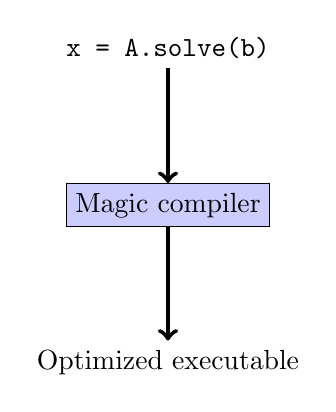
\begin{tikzpicture}
    \node (nprogram) at (0, 2) {\tt x = A.solve(b)};
    \node (ncompile) at (0, 0) [fill=blue!20,draw=black] {Magic compiler};
    \node (nresult)  at (0,-2) {Optimized executable};
    
    \draw [ultra thick,->] (nprogram) -- (ncompile);
    \draw [ultra thick,->] (ncompile) -- (nresult);
  \end{tikzpicture}
  \end{center}
\end{frame}


\begin{frame}
  \frametitle{Nerdvana?}

  \begin{center}
  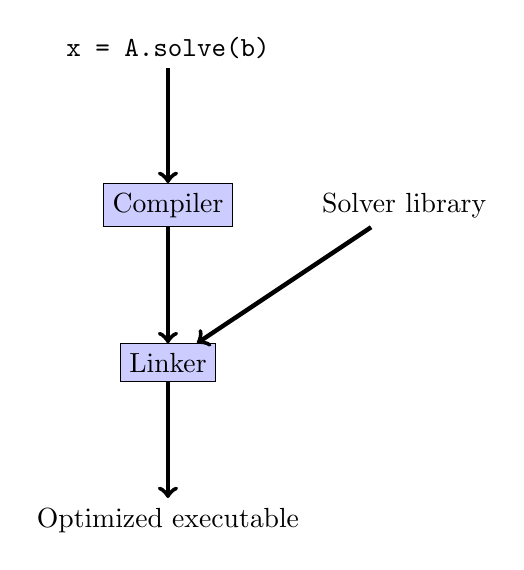
\begin{tikzpicture}
    \node (nprogram) at (0, 2) {\tt x = A.solve(b)};
    \node (nlibrary) at (3, 0) {Solver library};
    \node (ncompile) at (0, 0) [fill=blue!20,draw=black] {Compiler};
    \node (nlinker)  at (0,-2) [fill=blue!20,draw=black] {Linker};
    \node (nresult)  at (0,-4) {Optimized executable};
    
    \draw [ultra thick,->] (nprogram) -- (ncompile);
    \draw [ultra thick,->] (ncompile) -- (nlinker);
    \draw [ultra thick,->] (nlibrary) -- (nlinker);
    \draw [ultra thick,->] (nlinker) -- (nresult);
  \end{tikzpicture}
  \end{center}
\end{frame}


\begin{frame}
  \frametitle{Wait, what?}

  \begin{itemize}
  \item {\em Compiler} maps source code to assembly
  \item {\em Assembler} maps to object files
  \item {\em Librarian} produces
    \begin{itemize}
    \item Static {\em archives} ({\tt .a})
    \item Dynamic libraries or {\em shared objects} ({\tt .so})
    \end{itemize}
  \item {\em Linker} combines objects and resolves symbols
  \item {\em Loader} brings executable into memory
  \end{itemize}
  Usually worry about compile and link.
\end{frame}


\begin{frame}[fragile]
  \frametitle{Wait, what?}

  Consider calling LAPACK from C++.
\begin{lstlisting}
  extern "C"
  int dgesv_(const int& n, const int& nrhs,
             double* A, const int& ldA, int* ipiv,
             double* B, const int& ldB, int& info);

  ...
  dgesv_(n,1, A,n,ipiv, b,n, info);
  if (info != 0)
     complain_bitterly();
\end{lstlisting}
  Need to understand LAPACK conventions,
  name mangling (C++ and Fortran),
  calling conventions (by value/reference),
  one-vs-zero-base indexing ({\tt ipiv}), ...

  \vspace{2mm}
  NB: Can circumvent some with {\tt iso\_c\_binding} wrapper
\end{frame}


\begin{frame}[fragile]
  \frametitle{Wait, what?}

  Consider calling LAPACK from C++.
\begin{lstlisting}
 mycode.x: mycode.o
  g++ -o mycode.x mycode.o \
    -llapack -lopenblas -lgfortran -lm
  
mycode.o: mycode.cc
  g++ -c -O2 mycode.cc
\end{lstlisting}
  Need to understand inter-library dependencies, role of order on link
  line, role of front-end in bringing in language support libraries, ...

  \vspace{2mm}
  NB: Using wrapper libraries may not make this part simpler...
\end{frame}


\begin{frame}[fragile]
  \frametitle{Nerdvana?}

  \begin{lstlisting}
    x = A\b;
  \end{lstlisting}
\end{frame}


\begin{frame}[fragile]
  \frametitle{The mortal realm}

\begin{lstlisting}
umfpack_di_symbolic(n, n, Ap, Ai, Ax, &Symbolic,
                    NULL, NULL);
umfpack_di_numeric(Ap, Ai, Ax, Symbolic, &Numeric,
                    NULL, NULL);
umfpack_di_free_symbolic(&Symbolic);
umfpack_di_solve(UMFPACK_A, Ap, Ai, Ax, x, b, Numeric,
                 NULL, NULL);
umfpack_di_free_numeric(&Numeric);    
\end{lstlisting}
\end{frame}


\begin{frame}
  \frametitle{Hell}
  
  Write and tune a parallel sparse direct solver (in assembly?)
\end{frame}


\begin{frame}
  \frametitle{The mountain of abstraction}

  Consider the trajectory of the class:
  \begin{itemize}
  \item Started very low-level (caches, vector units, etc)
  \item Up to general ideas/kernels (tiling, matrix multiply)
  \item Up to parallel concepts, application ideas
  \item Nirvana: high-level code, performance ``just happens?''
  \end{itemize}
  Maybe the grass is greener across the C...
\end{frame}


\begin{frame}
  \frametitle{Low-level frameworks and languages}

  \begin{itemize}
  \item OpenMP and MPI (of course)
  \item Intel Thread Building Blocks (TBB)
  \item Global arrays
  \item Newer (?) parallel languages and extensions
    \begin{itemize}
    \item Cilk++
    \item UPC++
    \item Titanium
    \item Chapel
    \end{itemize}
  \end{itemize}
\end{frame}


\begin{frame}
  \frametitle{Libraries}

  One thing (or a few) done fast:
  \begin{itemize}
  \item BLAS (MKL, OpenBLAS, ATLAS, etc)
  \item LAPACK and successors
  \item FFTW
  \item Sparse direct solvers
  \end{itemize}
  Key challenge: linking (esp across languages)
\end{frame}


\begin{frame}
  \frametitle{Framework libraries}

  \begin{itemize}
  \item Many in PDE land
    \begin{itemize}
    \item PETSc, SLEPc, TAO, etc
    \item Trilinos
    \item Overture
    \item deal.ii
    \end{itemize}
  \item Interface more complicated than procedure call
  \item Effectively defines embedded solver language
  \end{itemize}
  Key challenge: learning framework + build/link
\end{frame}


\begin{frame}
  \frametitle{Runtime frameworks}

  \begin{itemize}
  \item Lots of trendy examples
    \begin{itemize}
    \item MapReduce / Hadoop
    \item Pregel, GraphLab, PowerGraph, Ligra, etc
    \item Spark
    \end{itemize}
  \item Write code to match interface desired by framework
  \item Promise: ``Code like this, we'll make it go fast''
    \begin{itemize}
    \item Great when it works!
    \item Sometimes not as fast as you'd hope
    \end{itemize}
  \end{itemize}
  Key challenge: map your problem to desired form

\end{frame}


\begin{frame}
  \frametitle{Scripting languages and PSEs}

  \begin{itemize}
  \item Matlab, Octave, R, Python, Julia
  \item ``High productivity'' vs ``high performance''?
  \item Not necessarily slow!
    \begin{itemize}
    \item Speed via extensions (Cython, MWrap, etc)
    \item Speed via Jit (Matlab, Julia, Python Numba)
    \item Speed via BLAS3 calls (all of the above)
    \item Often some parallel support as well
    \end{itemize}
  \item Performance strategies transfer
    \begin{itemize}
    \item Model and understand data access
    \item Profile and tune
    \end{itemize}
  \item Bottlenecks may not be where you expect
  \end{itemize}
  Key challenge: map your problem to fit language strengths
\end{frame}


\begin{frame}
  \frametitle{Domain specific languages}

  \begin{itemize}
  \item Classic example: SQL
  \item PDE domain: finite element compilers
    \begin{itemize}
    \item Dolfin framework
    \item Sundance
    \end{itemize}
  \item Embedded languages/specializers (PyCUDA, SEJITS)
  \end{itemize}
  Key challenge: great opportunities from limited scope
\end{frame}


\begin{frame}
  \frametitle{Simulation codes}

  \begin{itemize}
  \item ANSYS, ABAQUS, LS-DYNA, OpenSEES, FEAP, COMSOL, FLUENT,
    OpenFOAM, SPICE, Cadence, BioSPICE, ...
  \item Typical pattern
    \begin{itemize}
    \item Custom language (or preprocessor) for problem input
    \item Scripting language to describe analysis
    \item User-defined elements/modules in compiled language
    \end{itemize}
  \item Great for some classes of problems
  \item Can often be tortured into covering other types!
  \end{itemize}
  Key challenge: limited scope
\end{frame}


\begin{frame}
  \frametitle{High performance + high productivity?}

\end{frame}


\begin{frame}
  \frametitle{Warning: Strong opinion ahead!}

  Scripting is one of my favorite hammers!
  \begin{itemize}
  \item Used in my high school programming job
  \item And in my undergrad research project (tkbtg)
  \item And in early grad school (SUGAR)
  \item And later (FEAPMEX, HiQLab, BoneFEA)
  \end{itemize}

  \vspace{5mm}
  I think this is the Right Way to do a lot of things. \\
  But the details have changed over time.
\end{frame}


\begin{frame}[fragile]
  \frametitle{The rationale}

  Why is MATLAB nice?
  \begin{itemize}
  \item Conciseness of codes
  \item Expressive notation for matrix operations
  \item Interactive environment
  \item Rich set of numerical libraries
  \end{itemize}
  ... and codes rich in matrix operations are still fast!
\end{frame}


\begin{frame}
  \frametitle{The rationale}

  Typical simulations involve:
  \begin{itemize}
  \item Description of the problem parameters
  \item Description of solver parameters (tolerances, etc)
  \item Actual solution
  \item Postprocessing, visualization, etc
  \end{itemize}
  
  \vspace{5mm}
  What needs to be fast?
  \begin{itemize}
  \item Probably the solvers
  \item Probably the visualization
  \item Maybe not reading the parameters, problem setup?
  \end{itemize}

  \vspace{5mm}
  So save the C/Fortran coding for the solvers, visualization, etc.

\end{frame}


\begin{frame}
  \frametitle{Scripting uses}

  Use a mix of languages, with scripting languages to
  \begin{itemize}
  \item Automate processes involving multiple programs
  \item Provide more pleasant interfaces to legacy codes
  \item Provide simple ways to put together library codes
  \item Provide an interactive environment to play
  \item Set up problem and solver parameters
  \item Set up concise test cases
  \end{itemize}
  
  \vspace{5mm}
  Other stuff can go into the compiled code.

\end{frame}


\begin{frame}
  \frametitle{Smorgasbord of scripting}

  There are {\em lots} of languages to choose from.
  \begin{itemize}
  \item MATLAB, LISPs, Lua, Ruby, Python, Perl, ...
  \end{itemize}

  \vspace{1cm}
  For purpose of discussion, we'll use Python:
  \begin{itemize}
  \item Concise, easy to read
  \item Fun language features (classes, lambdas, keyword args)
  \item Freely available with a flexible license
  \item Large user community (including at national labs)
  \item ``Batteries included'' (including SciPy, matplotlib, Vtk, ...)
  \end{itemize}
\end{frame}


\begin{frame}
  \frametitle{Truth in advertising}

  Why haven't we been doing this in class so far?
  There are some not-always-simple issues:
  \begin{itemize}
  \item How do the languages communicate?
  \item How are extension modules compiled and linked?
  \item What support libraries are needed?
  \item Who owns the main loop?
  \item Who owns program objects?
  \item How are exceptions handled?
  \item How are semantic mismatches resolved?
  \item Does the interpreter have global state?
  \end{itemize}

  \vspace{5mm}
  Still worth the effort!
\end{frame}


\begin{frame}
  \frametitle{Simplest scripting usage}

  \begin{itemize}
  \item Script to prepare input files
  \item Run main program on input files
  \item Script for postprocessing output files
  \item And maybe some control logic
  \end{itemize}

  \vspace{1cm}
  This is portable, provides clean separation, but limited.
  
\end{frame}


\begin{frame}
  \frametitle{Scripting with IPC}

  \begin{itemize}
  \item Front-end written in a scripting language
  \item Back-end does actual computation
  \item Two communicate using some simple protocol 
    via inter-process communication (e.g. UNIX pipes)
  \end{itemize}

  \vspace{1cm}
  This is the way many GUIs are built.  Again, clean separation;
  somewhat less limited than communication via filesystem.  Works
  great for Unix variants (including OS X), but there are issues with
  IPC mechanism portability, particularly to Windows.

\end{frame}


\begin{frame}
  \frametitle{Scripting with RPC}

  \begin{itemize}
  \item Front-end client written in a scripting language
  \item Back-end server does actual computation
  \item Communicate via {\em remote procedure calls}
  \end{itemize}

  \vspace{1cm}
  This is how lots of web services work now (JavaScript in browser
  invoking remote procedure calls on server via SOAP).  Also idea
  behind CORBA, COM, etc.  There has been some work on variants for
  scientific computing.

\end{frame}


\begin{frame}
  \frametitle{Cross-language calls}

  \begin{itemize}
  \item Interpreter and application libraries in same executable
  \item Communication is via ``ordinary'' function calls
  \item Calls can go either way, either extending the interpreter
    or extending the application driver.  Former is usually easier.
  \end{itemize}

  \vspace{1cm}
  This has become the way a lot of scientific software is built ---
  including parallel software.  We'll focus here.

\end{frame}


\begin{frame}
  \frametitle{Concerning cross-language calls}
  
  What goes on when crossing language boundaries?
  \begin{itemize}
  \item Marshaling of argument data (translation+packaging)
  \item Function lookup
  \item Function invocation
  \item Translation of return data
  \item Translation of exceptional conditions
  \item Possibly some consistency checks, book keeping
  \end{itemize}

  For some types of calls (to C/C++/Fortran), automate this
  with {\em wrapper generators} and related tools.
\end{frame}


\begin{frame}
  \frametitle{Wrapper generators}

  Usual method: process interface specs
  \begin{itemize}
  \item Examples: SWIG, luabind, f2py, ...
  \item Input: an interface specification (e.g. cleaned-up header)
  \item Output: C code for gateway functions to call the interface
  \end{itemize}

  \vspace{5mm}
  Alternate method: language extensions
  \begin{itemize}
  \item Examples: weave, cython/pyrex, mwrap
  \item Input: script augmented with cross-language calls
  \item Output: normal script + compiled code (maybe just-in-time)
  \end{itemize}
\end{frame}


\begin{frame}[fragile]
  \frametitle{Example: {\tt mwrap} interface files}

Lines starting with \verb|#| are translated to C calls.
\begin{lstlisting}
function [qobj] = eventq();
  qobj = [];
  # EventQueue* q = new EventQueue();
  qobj.q = q;
  qobj = class(qobj, 'eventq');

function [e] = empty(qobj)
  q = qobj.q;
  # int e = q->EventQueue.empty();
\end{lstlisting}

\end{frame}

\begin{frame}[fragile]
  \frametitle{Example: SWIG interface file}

The SWIG input:
\begin{lstlisting}
%module ccube
%{
extern int cube( int n );
%}
int cube(int n);
\end{lstlisting}

\vspace{5mm}
Example usage from Python:
\begin{lstlisting}
import ccube
print "Output (10^3): ", ccube.cube(10)
\end{lstlisting}
\end{frame}


\begin{frame}[fragile]
  \frametitle{Is that it?}

{\small
\begin{lstlisting}
INC= /Library/Frameworks/Python.framework/Headers

example.o: example.c
        gcc -c $<

example_wrap.c: example.i
        swig -python example.i

example_wrap.o: example_wrap.c
        gcc -c -I$(INC) $<

_example.so: example.o example_wrap.o
        ld -bundle -flat_namespace \
           -undefined suppress -o $@ $^
\end{lstlisting}}
This is a Makefile from my laptop.  Must be a better way!

\end{frame}

\begin{frame}[fragile]
  \frametitle{A better build?}

\begin{lstlisting}
#! /usr/bin/env python
# setup.py

from distutils.core import *
from distutils      import sysconfig

_example = Extension( "_example",
                      ["example.i","example.c"])

setup( name        = "cube function",
       description = "cubes an integer",
       author      = "David Bindel",
       version     = "1.0",
       ext_modules = [_example] )
\end{lstlisting}
Run {\tt python setup.py build} to build.

\end{frame}


\begin{frame}
  \frametitle{The build problem}

  Actually figuring out how to build the code is hard!
  \begin{itemize}
  \item Hard to figure out libraries, link lines
  \item Gets harder when multiple machines are involved
  \item Several partial solutions
    \begin{itemize}
    \item {\tt pkg-config} is great (where it applies)
    \item CMake looks promising
    \item SCons was a contender
    \item Python distutils helps
    \item autotools are the old chestnut
    \item RTFM (when all else fails?)
    \end{itemize}
  \item Getting things to play nice is basis of some businesses!
  \end{itemize}

  \vspace{5mm}
  This is another reason to seek a large user community.

\end{frame}


\begin{frame}
  \frametitle{Brute-forcing the build problem}

  Idea:
  \begin{itemize}
  \item Figure out how to build on one Linux setup
  \item Capture key dependencies
  \item Encode in a virtual machine or Docker container
  \end{itemize}
  Pro: Everyone uses the same libraries, etc. \\
  Con: How does a generic build use specialized HW?

  \vspace{5mm}
  I suspect this will be how I teach this stuff in a couple years...
\end{frame}


\begin{frame}
  \frametitle{Mixed languages: tech issues}

  Primary technical pain points for mixed language code:
  \begin{itemize}
  \item Cross-language communication (wrapper generators help)
  \item Building and deployment (CMake and Docker help)
  \item Debugging and run-time issues (knowing what you're doing
    helps)
  \end{itemize}
\end{frame}


\begin{frame}
  \frametitle{Mixed languages: social issues}

  Primary sociological issues for (mixed) language adoption:
  \begin{itemize}
  \item Availability of learning resources and documentation
  \item Availability of support tools and libraries
  \item Active user base
  \item Open-ness of code base?
  \item Longevity
  \end{itemize}
\end{frame}


\begin{frame}
  \frametitle{A concluding thought}

  \begin{quote}
I don't know what the programming language of the year 2000 will look
like, but I know it will be called FORTRAN. \\
\hfill --- C.A.R.~Hoare
  \end{quote}
\end{frame}

% Technical issues for mixed language codes:
% - Cross-language communication
% - Building and deployment
% - Debugging and run-time issues (e.g. compatibility of exceptions?)

% Sociological issues for mixed language codes:
% - Learning resources
% - Infrastructure support and development + company support (libs, tools)
% - Active user base
% - Open code base?
% - Maintainability and tool longevity


\end{document}
